% !Mode:: "TeX:UTF-8"

\titlepage

\begin{frame}{说在前面}
	\linespread{1.5}
	  \begin{itemize}[<+-|alert@+>]
	    \item \ba{箭头!箭头!箭头!}
	    \item \ba{画图!画图!画图!}
	    \item 不记得自己哪周交作业
	  \end{itemize}
\end{frame}

% \begin{frame}{需要注意的问题}
% 	\linespread{1.5}
% 	  \begin{itemize}%[<+-|alert@+>]
% 	    \item L'Hospital法则
% 	    \begin{itemize}
% 	      \item \it 只能应用于“$\df{\bm{0}}{\bm{0}}$”
% 	      和“$\df{\bm{\infty}}{\bm{\infty}}$”型
% 	      \item \it 及时使用无穷小代换进行简化
% 	      \item \it 不正规的符号:\b 
% 	      $\xlongequal{\footnotesize\mbox{“L”}}$、
% 	      $\xlongrightarrow{\footnotesize\mbox{“L'Hospital法则”}}$、
% 	      $\df{\bm{0}}{\bm{0}}$、$\df{\bm{\infty}}{\bm{\infty}}$
% 	    \end{itemize}
% 	    \item Taylor公式
% 	    \begin{itemize}
% 	      \item \it Taylor多项式不包含余项
% 	      \item \it 合并同次幂的系数
% 	      \item \it 尽量按照幂次由低到高排列,最后写余项
% 	    \end{itemize}
% 	  \end{itemize}
% \end{frame}

\section{作业讲评:8.1 向量及其运算}

\begin{frame}
	\linespread{1.5}
	\ba{1.已知$(\bm{a}\times\bm{b})\cdot\bm{c}=2$,证明:
	$$[(\bm{a}+\bm{b})\times(\bm{b}+\bm{c})]\cdot(\bm{c}+\bm{a})=4$$.}
	
	\bigskip
	
	\small 解:\it
	略!
	
	\alert{注意叉乘满足反交换律!}
\end{frame}

\begin{frame}
	\linespread{1.5}
	\ba{2.求向量$\bm{a}=(4,3,4)$在向量$\bm{b}=(2,-2,1)$上的投影长度
	及投影向量。}
	
% 	\bigskip
	
	\small 解:\it
	$\bm{a}$在$\bm{b}$上的投影长度为
	$$(\bm{a})_{\bm{b}}=\df{\bm{a}\cdot\bm{b}}{|\bm{b}|}
	=2.$$
	$\bm{b}$对应的单位向量为
	$$\bm{e}_{\bm{b}}=\df{\bm{b}}{|\bm{b}|}=\left(\df23,-\df23,\df13\right),$$
	于是$\bm{a}$在$\bm{b}$上的投影向量为
	$$(\bm{a})_{\bm{b}}\cdot\bm{e}_{\bm{b}}=\left(\df43,-\df43,\df23\right).$$
	\fin
\end{frame}

\begin{frame}
	\linespread{1.5}
	\ba{3.设$\bm{a},\bm{b}$均为非零向量,且$|\bm{b}|=1$,二者夹角为$\pi/3$,求
	$\limx{0}\df{|\bm{a}+x\bm{b}|-|\bm{a}|}{x}$。}
	
	\bigskip
	
	\small 解:\it
	\begin{align*}
		&\limx{0}\df{|\bm{a}+x\bm{b}|-|\bm{a}|}{x}
		=\limx{0}\df{|\bm{a}+x\bm{b}|^2-|\bm{a}|^2}{x(|\bm{a}+x\bm{b}|+|\bm{a}|)}\\
		&=\limx{0}\df{(\bm{a}+x\bm{b})\cdot(\bm{a}+x\bm{b})
		-\bm{a}\cdot\bm{a}}{2x|\bm{a}|}
		=\limx{0}\df{2x\bm{a}\cdot\bm{b}+x^2|\bm{b}|^2}{2x|\bm{a}|}\\
		&=\df{\bm{a}\cdot\bm{b}}{|\bm{a}|}=|\bm{b}|\cos\df{\pi}3=\df12
	\end{align*}
	\fin
	
	\ba{注意:1、$\bm{a}$和$\bm{b}$未必是二维向量,不可以简单地假设其分量形式!
	2、没有$\bm{a}^2$这种形式!}
\end{frame}

\begin{frame}
	\linespread{1.5}
	\ba{4.已知平行四边形的两对角线向量分别为$\bm{A}=\bm{m}+2\bm{n}$,
	$\bm{B}=2\bm{m}-4\bm{n}$,其中$|\bm{m}|=1,|\bm{n}|=2$,
	$\bm{m}$和$\bm{n}$的夹角为$\pi/6$,求该平行四边形的面积。}
	
	\bigskip
	
	\small 解:\it
	以$\bm{A}$和$\bm{B}$为对角线的平行四边形面积,等于以$\bm{A}$和$\bm{B}$
	为相邻边的平行四边形面积的一半,故所求面积
	\begin{align*}
		S&=\df12{|\bm{A}\times\bm{B}|}
		=\df12|(\bm{m}+2\bm{n})\times(2\bm{m}-4\bm{n})|\\
		&=\df12|-6\bm{m}\times\bm{n}|
		=3|\bm{m}||\bm{n}|\sin\df{\pi}6=3.
	\end{align*}
	\fin
	
	\ba{注意:不要忘记取模!}
\end{frame}

\begin{frame}
	\linespread{1.5}
	\ba{5.画图:在空间直角坐标系中画出一个单位正立方体,然后在其表面上画出一个正六边形,
	{\it 使得六边形的每条边分别在六面体的一个面上}。}\pause
	
	\bigskip
	
	\begin{center}
		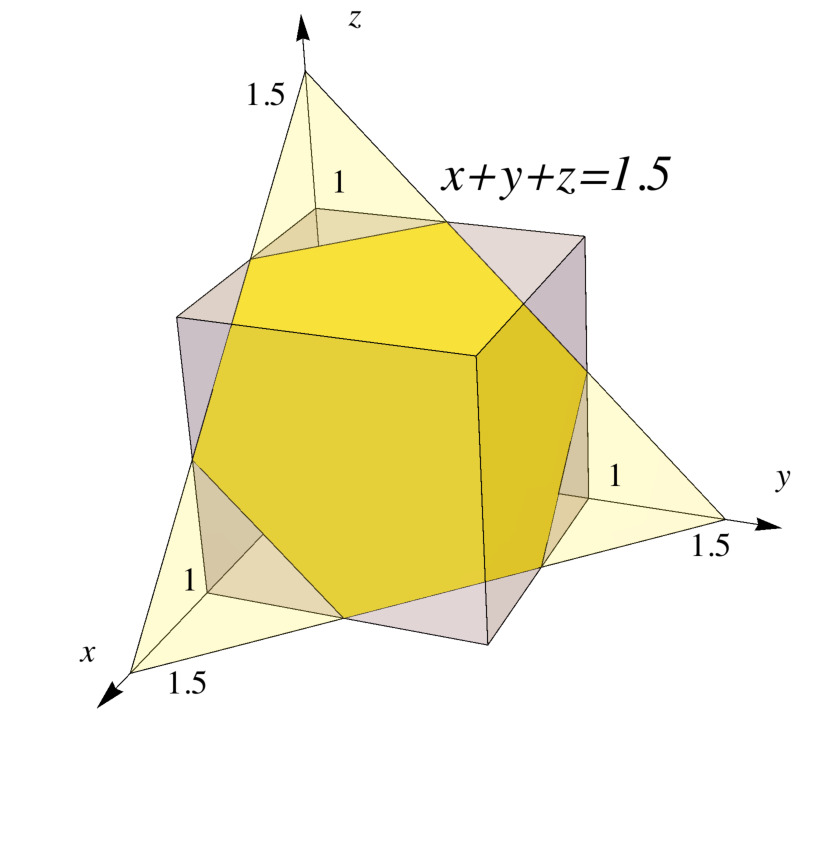
\includegraphics[width=0.5\textwidth]{./images/ch8/HexCubic.pdf}
	\end{center}
	\fin
\end{frame}

\begin{frame}
	\linespread{1.5}
	\ba{6.设向量$\bm{a},\bm{b},\bm{c}$不共面,向量
	$\bm{d}=\alpha\bm{a}+\beta\bm{b}+\gamma\bm{c}$,
	如果将$\bm{a},\bm{b},\bm{c},\bm{d}$的起点都放在一起,
	参数$\alpha,\beta,\gamma$须满足什么条件,方能使其终点在同一个平面上? }
	
	\bigskip
	
	\begin{columns}
		\begin{column}{.5\textwidth}
			\begin{center}
				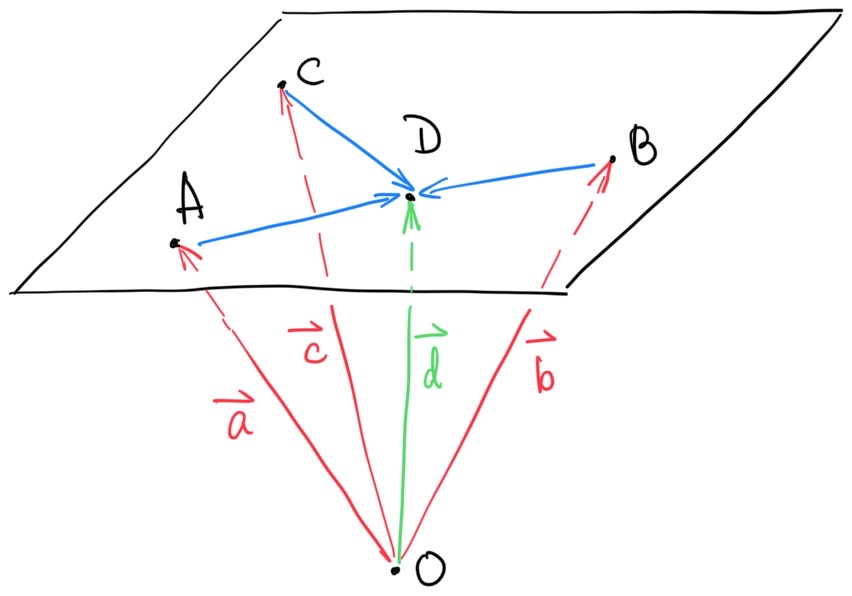
\includegraphics[width=.9\textwidth]{./images/ch8/abcd.jpg}
		% 		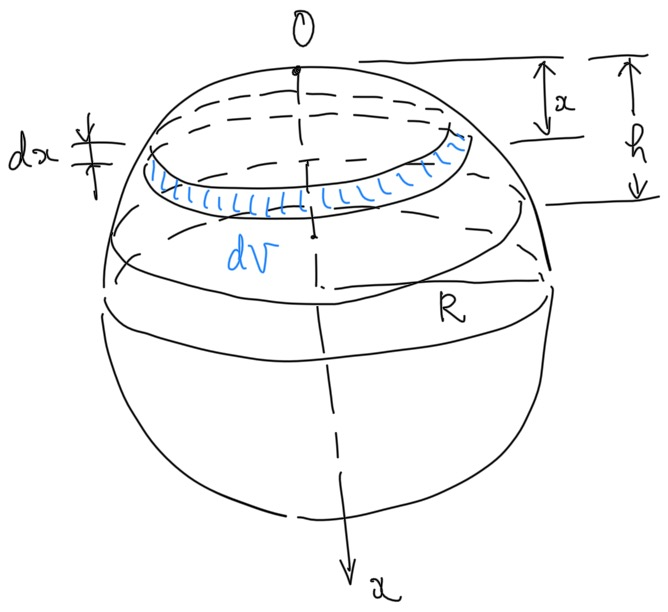
\includegraphics[width=6cm]{./images/ch6/topSp.jpg}
			\end{center}
		\end{column}
		\begin{column}{.5\textwidth}
			\small 解:\it
			由混合积的几何意义,点$A,B,C,D$共面当且仅当
			$$[(\bm{d}-\bm{a})\times(\bm{d}-\bm{b})]\cdot(\bm{d}-\bm{c})=0,$$
			利用向量运算的性质化简,最后可得$\alpha+\beta+\gamma=1$。\fin
		\end{column}
	\end{columns}
\end{frame}

\section{补充例题}

\begin{frame}{判断}
	\linespread{1.2}
	\begin{enumerate}
	  \item $\bm{a}\cdot\bm{a}\cdot\bm{a}=\bm{a}^3$\quad\pause\ba{$\times$}\pause
	  \item $\bm{a}\ne 0$时,$\df{\bm{a}}{\bm{a}}=1$\quad\pause\ba{$\times$}\pause
	  \item $\bm{a}(\bm{a}\cdot\bm{b})=\bm{a}^2\bm{b}$
	    \quad\pause\ba{$\times$}\pause
	  \item $(\bm{a}\cdot\bm{b})^2=\bm{a}^2\bm{b}^2$\quad\pause\ba{$\times$}\pause
	  \item $|\bm{a}\cdot\bm{b}|=|\bm{a}|\cdot|\bm{b}|$
		\quad\pause\ba{$\times$}\pause
	  \item $(\bm{a}+\bm{b})\times(\bm{a}-\bm{b})=\bm{a}\times\bm{a}
  		-\bm{b}\times\bm{b}=0$
  		\quad\pause\ba{$\times$}\pause
  	  \item $\bm{a}\ne 0$时,$\bm{a}\cdot\bm{b}
  	  	=\bm{a}\cdot\bm{c}\Rightarrow\bm{b}=\bm{c}$
  	  	\quad\pause\ba{$\times$}\pause
  	  \item  $\bm{a}\ne 0$时,$\bm{a}\times\bm{b}
  	  	=\bm{a}\times\bm{c}\Rightarrow\bm{b}=\bm{c}$
  	  	\quad\pause\ba{$\times$}
	\end{enumerate}
\end{frame}

\begin{frame}{填空}
	\linespread{1.2}
	
	\ba{1.}\;设$\bm{a},\bm{b}$均为非零向量,则
	其角平分线上的向量为
	\underline{\uncover<2->{\;\b{$C\left(\df{\bm{a}}{|\bm{a}|}
	+\df{\bm{b}}{|\bm{b}|}\right),\;(C\in\mathbb{R})$}}\;}.\\[1em]
	
	\ba{2.}\;设$\bm{a},\bm{b},\bm{c}$均为非零向量,且$\bm{a}=\bm{b}\times\bm{c}$,
	$\bm{b}=\bm{c}\times\bm{a}$,
	$\bm{c}=\bm{a}\times\bm{b}$则
	$|\bm{a}|+|\bm{b}|+|\bm{c}|=$
	\underline{\uncover<3->{\;\b{$3$}}\;}.\\[1em]

	\ba{3.}\;设$|\bm{a}|=2,|\bm{b}|=2$,$\bm{a}$和$\bm{b}$
	的夹角为$\pi/3$,则$|2\bm{a}-3\bm{b}|=$
	\underline{\uncover<4->{\;\b{$2\sqrt7$}}\;}.\\[1em]
		
	\ba{4.}\;平面$Ax+By+Cz+D_i=0\;(i=1,2)$之间的距离为
	\underline{\uncover<5->{\;\b{$\df{|D_1-D_2|}{\sqrt{A^2+B^2+C^2}}$}}\;}.
\end{frame}

\begin{frame}{选择}
	\linespread{1.3}
	\ba{1.}\;设$\bm{a},\bm{b},\bm{c}$均为非零向量,则与$\bm{a}$不垂直的是
	(\underline{\uncover<2->{\;\b{D}}\;})
	\begin{enumerate}[(A)]
	  \item $(\bm{a}\cdot\bm{c})\bm{b}-(\bm{a}\cdot\bm{b})\bm{c}$
	  \item $\bm{b}-\left(\df{\bm{a}\cdot\bm{b}}{\bm{|a|}^2}\right)\bm{a}$
	  \item $\bm{a}\times\bm{b}$
	  \item $\bm{a}+(\bm{a}\times\bm{b})\times\bm{a}$
	\end{enumerate}
\end{frame}

\begin{frame}{选择}
	\linespread{1.3}
	\ba{2.}\;设$\bm{a},\bm{b}$为非零向量,$|\bm{a}-\bm{b}|=|\bm{a}+\bm{b}|$,则
	(\underline{\uncover<2->{\;\b{C}}\;})
	\begin{enumerate}[(A)]
	  \item $\bm{a}-\bm{b}=\bm{a}+\bm{b}$
	  \item $\bm{a}=\bm{b}$
	  \item $\bm{a}\cdot\bm{b}=0$
	  \item $\bm{a}\times\bm{b}=0$
	\end{enumerate}
\end{frame}

% \begin{frame}{选择}
% 	\linespread{1.3}
% 	\ba{3.}\;设$\bm{a},\bm{b}$为非零向量,且满足
% 	$(\bm{a}+3\bm{b})\perp(7\bm{a}-5\bm{b})$,
% 	$(\bm{a}-4\bm{b})\perp(7\bm{a}+2\bm{b})$,则
% 	向量$\bm{a}$和$\bm{b}$的夹角为
% 	(\underline{\uncover<2->{\;\b{C}}\;})
% 	\begin{enumerate}[(A)]
% 	  \item $0$
% 	  \item $\pi/2$
% 	  \item $\pi/3$
% 	  \item $2\pi/3$
% 	\end{enumerate}
% \end{frame}

\begin{frame}{选择}
	\linespread{1.3}
	\ba{3.}\;设平面$\pi$位于平面$x-2y+z-2=0$和$x-2y+z-6=0$之间,
	且与此二平面的距离之比为$1:3$,则$\pi$的方程为
	(\underline{\uncover<2->{\;\b{A}}\;})
	\begin{enumerate}[(A)]
	  \item $x-2y+z-5=0$或$x-2y+z-3=0$
	  \item $x-2y+z+8=0$
	  \item $x+2y+4z=0$
	  \item $x-2y+5z-3=0$
	\end{enumerate}
\end{frame}

\begin{frame}{选择}
	\linespread{1.3}
	\ba{4.}\;设$\left|\begin{array}{ccc}
	a_1 & b_1 & c_1\\ a_2 & b_2 & c_2\\ a_3 & b_3 & c_3
	\end{array}\right|\ne 0$,则
	直线
	$\df{x-a_3}{a_1-a_2}=\df{y-b_3}{b_1-b_2}$
	$=\df{z-c_3}{c_1-c_2}$
	和
	$\df{x-a_1}{a_2-a_3}=\df{y-b_1}{b_2-b_3}=\df{z-c_1}{c_2-c_3}$
	(\underline{\uncover<2->{\;\b{A}}\;})
	\begin{enumerate}[(A)]
	  \item 相交于一点
	  \item 重合
	  \item 平行但不重合
	  \item 异面直线
	\end{enumerate}
\end{frame}

\begin{frame}{解答}
	\linespread{1.2}
	\ba{1.}\;过原点且与
	$$\left\{\begin{array}{l}
	x=1\\ y=-1+t\\ z=2+t
	\end{array}\right.$$
	和$x+1=\df{y+2}2=z-1$都平行的平面方程。
	
	\pause\alert{提示:}\it\b  
	$$x-y+z=0$$
\end{frame}

\begin{frame}{解答}
	\linespread{1.2}
	\ba{2.}\;求过点$M(3,1,-2)$和直线$\df{x-4}5=\df{y+3}2=\df z1$
	的平面方程。
	
	\pause\ba{法一:}\it\b  
	$\bm{n}=\bm{s}\times\bm{MM_1}=(-8,9,22)$,平面方程
	$$8x-9y-22x-59=0$$
	
	\pause\ba{法二:}
	直线的一般式方程:$\left\{\begin{array}{l}x-5y-4=0\\ 
	y-2z+3=0\end{array}\right.$,建立平面束方程,进而可得$\lambda=8,\mu=-9$
\end{frame}

% \begin{frame}
% 	\linespread{1.2}
% 	\ba{3.}\;过直线
% 	$\df{x-1}2=\df{y+2}{-3}=\df{z-2}2$且垂直于平面
% 	$3x+2y-z=5$的平面方程。
% 	
% 	\pause\alert{提示:}{\b  
% 	$$x-8y-13z+9=0$$}
% 	
% 	\pause
% 	\ba{4.}\;求过直线
% 	$$\left\{\begin{array}{l}
% 		x+5y+z=0\\
% 		x-z+4=0
% 	\end{array}\right.$$
% 	且与平面$\pi:x-4y-8z+12=0$的夹角为$\pi/4$的平面方程。
% \end{frame}

\begin{frame}
	\linespread{1.2}
	\ba{3.}\;过点$(-1,0,4)$,平行于平面
	$3x-4y+z=10$,且与直线$x+1=y-3=\df z2$
	相交的直线方程。

	\pause\alert{提示:}\it\b 建立所求直线的参数方程,最终解得
	$$\df{x+1}{16}=\df{y}{19}=\df{z-4}{28}$$
\end{frame}

\begin{frame}
	\linespread{1.2}
	\ba{4.}\;已知$P(3,1,-4)$和$L:\df{x+1}2=\df{y-4}{-2}=z-1$,求
	\begin{enumerate}
	  \item $P$到$L$的距离;
	  \item $P$在$L$上的垂足$Q$的坐标;
	  \item 设$R(1,2,3)$在$L$上的垂足为$N$,求$QN$的长度。
	\end{enumerate}

	\pause\alert{提示:}\it\b
	$(1)\sqrt{41}$\quad$(2)(1,2,2)$\quad$(3)\df13$
\end{frame}

\begin{frame}
	\linespread{1.2}
	\ba{5.}\;已知直线
	$$L_1:\left\{\begin{array}{l}
		x+y+z+1=0\\
		2x-y+3z+4=0
	\end{array}\right.
	\quad
	L_2:\left\{\begin{array}{l}
		x=-1+2t\\
		y=-t\quad(t\in\mathbb{R})\\
		z=2-2t
	\end{array}\right.
	$$
	\begin{enumerate}[(1)]
% 	  \setlength{\itemindent}{1cm}
	  \item 证明两直线异面;
	  \item 求两直线间的距离;
	  \item 求二者的公垂线方程。
	\end{enumerate}
	
	\pause\alert{提示:}\it\b
	$L_1,L_2$的标准式方程
	$$\df{x+3}4=\df{y-1}{-1}=\df{z-1}{-3},\quad
	\df{x+1}2=\df y{-1}=\df{z-2}{-2}$$
\end{frame}

% \begin{frame}
% 	\linespread{1.2}
% 	\ba{8.}\;计算由以下平面所围成的立体体积:
% 	$$a_ix+b_iy+c_iz=\pm h_i,\;i=1,2,3,$$
% 	其中:$a_i,b_i,c_i$为常数,$h_i\ne0(i=1,2,3)$,且
% 	$$\Delta=\left|\begin{array}{ccc}
% 	a_1 & b_1 & c_1\\ a_2 & b_2 & c_2 \\ a_3 & b_3 & c_3
% 	\end{array}\right|\ne 0$$
% 	
% 	\pause\alert{提示:}\b
% 	$$\left[(\bm{s}_1\times\bm{s}_2)\times
% 	(\bm{s}_2\times\bm{s}_3)\right]\cdot(\bm{s}_3\times\bm{s}_1)=
% 	\left[(\bm{s}_1\times\bm{s}_2)\cdot\bm{s}_3\right]^2$$ 
% \end{frame}
% 
% \begin{frame}{讨论}
% 	\linespread{1.2}
% 	\begin{enumerate}
% 	  \item 证明:$\bm{s}_1\times(\bm{s}_2\times\bm{s}_3)
% 	  	=(\bm{s}_1\cdot\bm{s}_3)\bm{s}_2
% 		-(\bm{s}_1\cdot\bm{s}_2)\bm{s}_3$\pause
% 	  \item 证明:$\left[(\bm{s}_1\times\bm{s}_2)\times
% 	  	(\bm{s}_2\times\bm{s}_3)\right]
% 		\cdot(\bm{s}_3\times\bm{s}_1)
% 		=\left[(\bm{s}_1\times\bm{s}_2)\cdot\bm{s}_3\right]^2$\pause
% 	  \item $\bm{s}_1\times(\bm{s}_2\times\bm{s}_3)
% 	  =(\bm{s}_1\times\bm{s}_2)\times\bm{s}_3$成立吗?
% 	\end{enumerate}
% 	\ba{提示:}\it\b 反例:
% 	$$\bm{j}\times(\bm{i}\times\bm{i})=0$$
% 	$$(\bm{j}\times\bm{i})\times\bm{i}=-\bm{k}\times\bm{i}=-\bm{j}$$
% \end{frame}

% \begin{frame}{出现的问题}
% 	\linespread{1.5}
% 	  \begin{itemize}%[<+-|alert@+>]
% 	    \item 作业进度慢!
% 	    \item 概念问题
% 	    \begin{itemize}
% 	      \item \b\it 幂级数展开不熟练
% 	      \item \b\it Maclaurin级数和关于$(x-x_0)$的幂级数分不清
% 	    \end{itemize}
% 	    \item 过程不规范或不完整
% 	    \begin{itemize}
% 	      \item \b\it 求收敛域要单独讨论端点的敛散性
% 	      \item \b\it 相同幂次的项要合并,并按幂次从小到大排列
% 	      \item \b\it 书写潦草随意\pause
% 	    \end{itemize}
% 	    \item \ba{雷同!!!}
% 	  \end{itemize}
% \end{frame}

% \begin{frame}
% 	\linespread{1.5}
% 	\ba{3.设$D$是由曲线$y=\sin x+1$与三条直线$x=0,x=\pi,y=0$
% 	所围成的曲边梯形,求$D$绕$x$轴旋转一周所围成的旋转体的体积。
% 	}
% 	\pause
% 	
% % 	\bigskip
% 	
% 	\begin{columns}
% 		\begin{column}{.5\textwidth}
% 			\begin{center}
% 				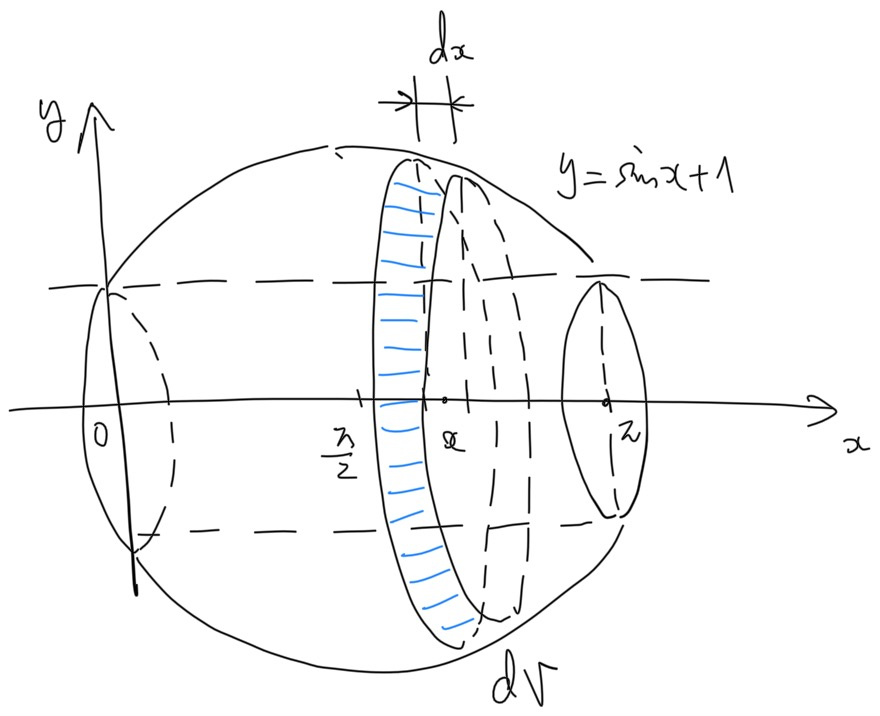
\includegraphics[width=.9\textwidth]{./images/ch6/sinx1cs.jpg}
% 		% 		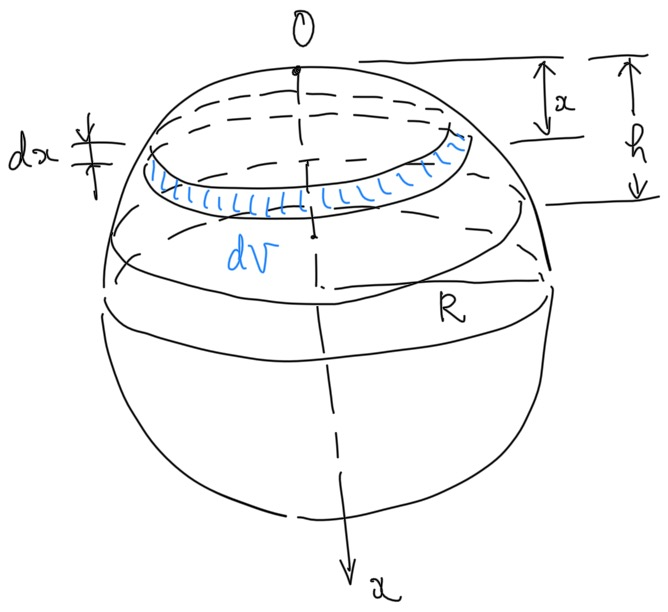
\includegraphics[width=6cm]{./images/ch6/topSp.jpg}
% 			\end{center}		
% 		\end{column}
% 		\begin{column}{.5\textwidth}
% 			\small 解:\it
% 			如图,体积微元$\d V=\pi y^2\d x$,	故所求体积
% 			$$
% 				V=\dint_0^{\pi}\pi(\sin x+1)^2\d x=\df32\pi^2.
% 			$$
% 		\end{column}
% 	\end{columns}
% \end{frame}